\subsection{幅の証拠}

図~\ref{fig:width}は、文献・インスタンス別に抽出した幅の値を示す。
幅は、既存研究がどの程度の問題規模を量子回路へ写像しているかを示す。
小規模シミュレーションや実機デモでは数十量子ビット級の例が多い一方、資源推定ではより多くの量子ビットが要求されることが示されている。

\begin{figure}[t]
  \centering
  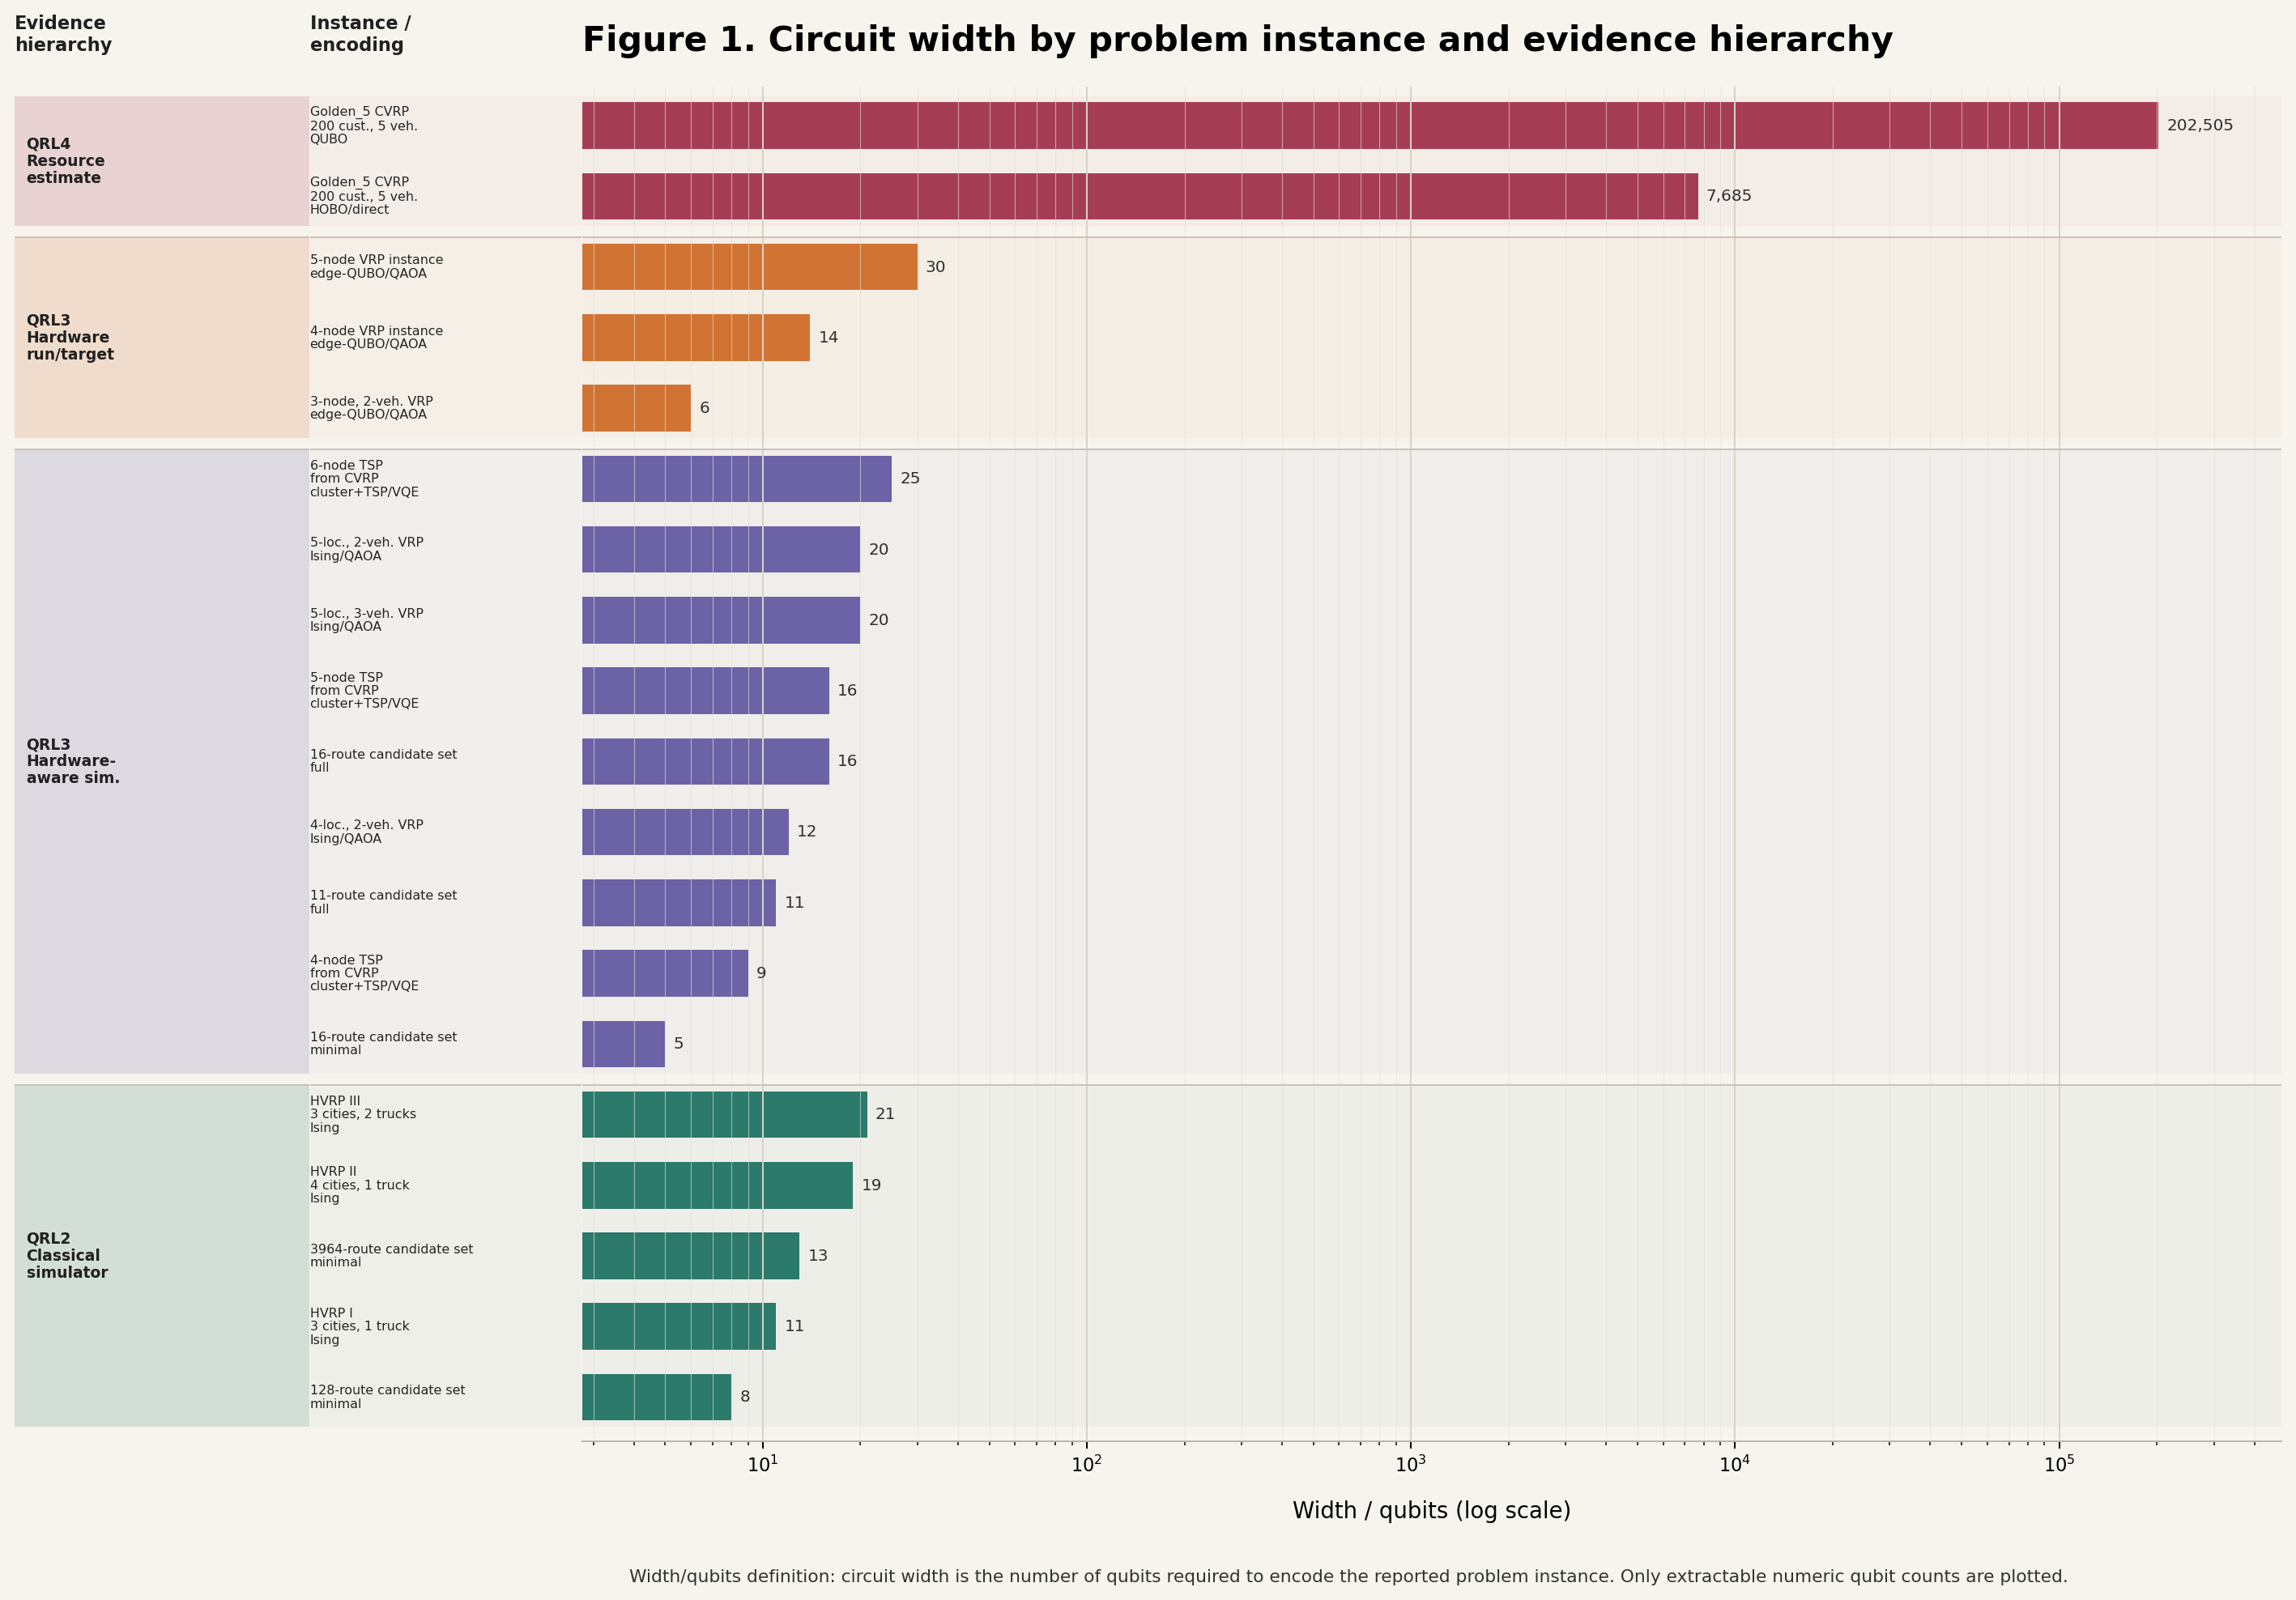
\includegraphics[width=0.95\linewidth]{../06_outputs/figures/active/01_quantum_vrp_evidence/figure_1_width_by_instance.png}
  \caption{文献・インスタンス別の回路幅}
  \label{fig:width}
\end{figure}

\subsection{深さの証拠}

深さは論文ごとに意味が異なるため、独立した図として単純比較しない。
本研究では、QAOA層、ansatz layer、理論深さ、トランスパイル後のgate countを区別し、Table~\ref{tab:gap-matrix}の解釈上の注意として扱う。

\subsection{ギャップ表}

既存文献と社会・技術ロードマップの間には、少なくとも規模ギャップ、資源ギャップ、ハードウェア・ワークフローギャップ、実行可能性ギャップ、幅・深さのトレードオフがある。
表~\ref{tab:gap-matrix}は、これらのギャップを要約する。

\begin{table}[t]
\centering
\caption{段階ベースのギャップ表}
\label{tab:gap-matrix}
\begin{tabular}{p{0.22\linewidth}p{0.68\linewidth}}
\toprule
ギャップ & 解釈 \\
\midrule
規模ギャップ & 既存VRP-QAOA研究は小規模実験中心であり、運用規模とは距離がある。 \\
資源ギャップ & 資源推定段階のCVRPでは、実用候補規模がNISQの幅・深さを超える。 \\
ハードウェア・ワークフローギャップ & ショット数、実行時間、接続性、ノイズ、実行不可能状態が小規模実機実験でも制約になる。 \\
実行可能性ギャップ & 低い目的関数値ではなく、実行可能経路の取得を別ギャップとして扱う必要がある。 \\
幅・深さのトレードオフ & 量子ビット効率の高い符号化は幅を減らし得るが、深さ、高次相互作用、測定、ワークフロー負担へ制約を移す可能性がある。 \\
\bottomrule
\end{tabular}
\end{table}
